%% bare_adv.tex
%% V1.4a
%% 2014/09/17
%% by Michael Shell
%% See: 
%% http://www.michaelshell.org/
%% for current contact information.
%%
%% This is a skeleton file demonstrating the advanced use of IEEEtran.cls
%% (requires IEEEtran.cls version 1.8a or later) with an IEEE Computer
%% Society journal paper.
%%
%% Support sites:
%% http://www.michaelshell.org/tex/ieeetran/
%% http://www.ctan.org/tex-archive/macros/latex/contrib/IEEEtran/
%% and
%% http://www.ieee.org/

%%*************************************************************************
%% Legal Notice:
%% This code is offered as-is without any warranty either expressed or
%% implied; without even the implied warranty of MERCHANTABILITY or
%% FITNESS FOR A PARTICULAR PURPOSE! 
%% User assumes all risk.
%% In no event shall IEEE or any contributor to this code be liable for
%% any damages or losses, including, but not limited to, incidental,
%% consequential, or any other damages, resulting from the use or misuse
%% of any information contained here.
%%
%% All comments are the opinions of their respective authors and are not
%% necessarily endorsed by the IEEE.
%%
%% This work is distributed under the LaTeX Project Public License (LPPL)
%% ( http://www.latex-project.org/ ) version 1.3, and may be freely used,
%% distributed and modified. A copy of the LPPL, version 1.3, is included
%% in the base LaTeX documentation of all distributions of LaTeX released
%% 2003/12/01 or later.
%% Retain all contribution notices and credits.
%% ** Modified files should be clearly indicated as such, including  **
%% ** renaming them and changing author support contact information. **
%%
%% File list of work: IEEEtran.cls, IEEEtran_HOWTO.pdf, bare_adv.tex,
%%                    bare_conf.tex, bare_jrnl.tex, bare_conf_compsoc.tex,
%%                    bare_jrnl_compsoc.tex, bare_jrnl_transmag.tex
%%*************************************************************************


% *** Authors should verify (and, if needed, correct) their LaTeX system  ***
% *** with the testflow diagnostic prior to trusting their LaTeX platform ***
% *** with production work. IEEE's font choices and paper sizes can       ***
% *** trigger bugs that do not appear when using other class files.       ***                          ***
% The testflow support page is at:
% http://www.michaelshell.org/tex/testflow/


% IEEEtran V1.7 and later provides for these CLASSINPUT macros to allow the
% user to reprogram some IEEEtran.cls defaults if needed. These settings
% override the internal defaults of IEEEtran.cls regardless of which class
% options are used. Do not use these unless you have good reason to do so as
% they can result in nonIEEE compliant documents. User beware. ;)
%
%\newcommand{\CLASSINPUTbaselinestretch}{1.0} % baselinestretch
%\newcommand{\CLASSINPUTinnersidemargin}{1in} % inner side margin
%\newcommand{\CLASSINPUToutersidemargin}{1in} % outer side margin
%\newcommand{\CLASSINPUTtoptextmargin}{1in}   % top text margin
%\newcommand{\CLASSINPUTbottomtextmargin}{1in}% bottom text margin




%
\documentclass[10pt,journal,compsoc]{IEEEtran}
% If IEEEtran.cls has not been installed into the LaTeX system files,
% manually specify the path to it like:
% \documentclass[10pt,journal,compsoc]{../sty/IEEEtran}


% For Computer Society journals, IEEEtran defaults to the use of 
% Palatino/Palladio as is done in IEEE Computer Society journals.
% To go back to Times Roman, you can use this code:
%\renewcommand{\rmdefault}{ptm}\selectfont





% Some very useful LaTeX packages include:
% (uncomment the ones you want to load)



% *** MISC UTILITY PACKAGES ***
%
%\usepackage{ifpdf}
% Heiko Oberdiek's ifpdf.sty is very useful if you need conditional
% compilation based on whether the output is pdf or dvi.
% usage:
% \ifpdf
%   % pdf code
% \else
%   % dvi code
% \fi
% The latest version of ifpdf.sty can be obtained from:
% http://www.ctan.org/tex-archive/macros/latex/contrib/oberdiek/
% Also, note that IEEEtran.cls V1.7 and later provides a builtin
% \ifCLASSINFOpdf conditional that works the same way.
% When switching from latex to pdflatex and vice-versa, the compiler may
% have to be run twice to clear warning/error messages.






% *** CITATION PACKAGES ***
%
\ifCLASSOPTIONcompsoc
  % IEEE Computer Society needs nocompress option
  % requires cite.sty v4.0 or later (November 2003)
  \usepackage[nocompress]{cite}
\else
  % normal IEEE
  \usepackage{cite}
\fi
% cite.sty was written by Donald Arseneau
% V1.6 and later of IEEEtran pre-defines the format of the cite.sty package
% \cite{} output to follow that of IEEE. Loading the cite package will
% result in citation numbers being automatically sorted and properly
% "compressed/ranged". e.g., [1], [9], [2], [7], [5], [6] without using
% cite.sty will become [1], [2], [5]--[7], [9] using cite.sty. cite.sty's
% \cite will automatically add leading space, if needed. Use cite.sty's
% noadjust option (cite.sty V3.8 and later) if you want to turn this off
% such as if a citation ever needs to be enclosed in parenthesis.
% cite.sty is already installed on most LaTeX systems. Be sure and use
% version 5.0 (2009-03-20) and later if using hyperref.sty.
% The latest version can be obtained at:
% http://www.ctan.org/tex-archive/macros/latex/contrib/cite/
% The documentation is contained in the cite.sty file itself.
%
% Note that some packages require special options to format as the Computer
% Society requires. In particular, Computer Society  papers do not use
% compressed citation ranges as is done in typical IEEE papers
% (e.g., [1]-[4]). Instead, they list every citation separately in order
% (e.g., [1], [2], [3], [4]). To get the latter we need to load the cite
% package with the nocompress option which is supported by cite.sty v4.0
% and later.





% *** GRAPHICS RELATED PACKAGES ***
%
\ifCLASSINFOpdf
\usepackage[pdftex]{graphicx}
  % declare the path(s) where your graphic files are
  % \graphicspath{{../pdf/}{../jpeg/}}
  % and their extensions so you won't have to specify these with
  % every instance of \includegraphics
  % \DeclareGraphicsExtensions{.pdf,.jpeg,.png}
\else
  % or other class option (dvipsone, dvipdf, if not using dvips). graphicx
  % will default to the driver specified in the system graphics.cfg if no
  % driver is specified.
  % \usepackage[dvips]{graphicx}
  % declare the path(s) where your graphic files are
  % \graphicspath{{../eps/}}
  % and their extensions so you won't have to specify these with
  % every instance of \includegraphics
  % \DeclareGraphicsExtensions{.eps}
\fi
% graphicx was written by David Carlisle and Sebastian Rahtz. It is
% required if you want graphics, photos, etc. graphicx.sty is already
% installed on most LaTeX systems. The latest version and documentation
% can be obtained at: 
% http://www.ctan.org/tex-archive/macros/latex/required/graphics/
% Another good source of documentation is "Using Imported Graphics in
% LaTeX2e" by Keith Reckdahl which can be found at:
% http://www.ctan.org/tex-archive/info/epslatex/
%
% latex, and pdflatex in dvi mode, support graphics in encapsulated
% postscript (.eps) format. pdflatex in pdf mode supports graphics
% in .pdf, .jpeg, .png and .mps (metapost) formats. Users should ensure
% that all non-photo figures use a vector format (.eps, .pdf, .mps) and
% not a bitmapped formats (.jpeg, .png). IEEE frowns on bitmapped formats
% which can result in "jaggedy"/blurry rendering of lines and letters as
% well as large increases in file sizes.
%
% You can find documentation about the pdfTeX application at:
% http://www.tug.org/applications/pdftex





% *** MATH PACKAGES ***
%
\usepackage[cmex10]{amsmath}
% A popular package from the American Mathematical Society that provides
% many useful and powerful commands for dealing with mathematics. If using
% it, be sure to load this package with the cmex10 option to ensure that
% only type 1 fonts will utilized at all point sizes. Without this option,
% it is possible that some math symbols, particularly those within
% footnotes, will be rendered in bitmap form which will result in a
% document that can not be IEEE Xplore compliant!
%
% Also, note that the amsmath package sets \interdisplaylinepenalty to 10000
% thus preventing page breaks from occurring within multiline equations. Use:
%\interdisplaylinepenalty=2500
% after loading amsmath to restore such page breaks as IEEEtran.cls normally
% does. amsmath.sty is already installed on most LaTeX systems. The latest
% version and documentation can be obtained at:
% http://www.ctan.org/tex-archive/macros/latex/required/amslatex/math/





% *** SPECIALIZED LIST PACKAGES ***
%\usepackage{acronym}
% acronym.sty was written by Tobias Oetiker. This package provides tools for
% managing documents with large numbers of acronyms. (You don't *have* to
% use this package - unless you have a lot of acronyms, you may feel that
% such package management of them is bit of an overkill.)
% Do note that the acronym environment (which lists acronyms) will have a
% problem when used under IEEEtran.cls because acronym.sty relies on the
% description list environment - which IEEEtran.cls has customized for
% producing IEEE style lists. A workaround is to declared the longest
% label width via the IEEEtran.cls \IEEEiedlistdecl global control:
%
% \renewcommand{\IEEEiedlistdecl}{\IEEEsetlabelwidth{SONET}}
% \begin{acronym}
%
% \end{acronym}
% \renewcommand{\IEEEiedlistdecl}{\relax}% remember to reset \IEEEiedlistdecl
%
% instead of using the acronym environment's optional argument.
% The latest version and documentation can be obtained at:
% http://www.ctan.org/tex-archive/macros/latex/contrib/acronym/


%\usepackage{algorithmic}
% algorithmic.sty was written by Peter Williams and Rogerio Brito.
% This package provides an algorithmic environment fo describing algorithms.
% You can use the algorithmic environment in-text or within a figure
% environment to provide for a floating algorithm. Do NOT use the algorithm
% floating environment provided by algorithm.sty (by the same authors) or
% algorithm2e.sty (by Christophe Fiorio) as IEEE does not use dedicated
% algorithm float types and packages that provide these will not provide
% correct IEEE style captions. The latest version and documentation of
% algorithmic.sty can be obtained at:
% http://www.ctan.org/tex-archive/macros/latex/contrib/algorithms/
% There is also a support site at:
% http://algorithms.berlios.de/index.html
% Also of interest may be the (relatively newer and more customizable)
% algorithmicx.sty package by Szasz Janos:
% http://www.ctan.org/tex-archive/macros/latex/contrib/algorithmicx/




% *** ALIGNMENT PACKAGES ***
%
%\usepackage{array}
% Frank Mittelbach's and David Carlisle's array.sty patches and improves
% the standard LaTeX2e array and tabular environments to provide better
% appearance and additional user controls. As the default LaTeX2e table
% generation code is lacking to the point of almost being broken with
% respect to the quality of the end results, all users are strongly
% advised to use an enhanced (at the very least that provided by array.sty)
% set of table tools. array.sty is already installed on most systems. The
% latest version and documentation can be obtained at:
% http://www.ctan.org/tex-archive/macros/latex/required/tools/


%\usepackage{mdwmath}
%\usepackage{mdwtab}
% Also highly recommended is Mark Wooding's extremely powerful MDW tools,
% especially mdwmath.sty and mdwtab.sty which are used to format equations
% and tables, respectively. The MDWtools set is already installed on most
% LaTeX systems. The lastest version and documentation is available at:
% http://www.ctan.org/tex-archive/macros/latex/contrib/mdwtools/


% IEEEtran contains the IEEEeqnarray family of commands that can be used to
% generate multiline equations as well as matrices, tables, etc., of high
% quality.


%\usepackage{eqparbox}
% Also of notable interest is Scott Pakin's eqparbox package for creating
% (automatically sized) equal width boxes - aka "natural width parboxes".
% Available at:
% http://www.ctan.org/tex-archive/macros/latex/contrib/eqparbox/




% *** SUBFIGURE PACKAGES ***
%\ifCLASSOPTIONcompsoc
% \usepackage[caption=false,font=footnotesize,labelfont=sf,textfont=sf]{subfig}
%\else
%  \usepackage[caption=false,font=footnotesize]{subfig}
%\fi
% subfig.sty, written by Steven Douglas Cochran, is the modern replacement
% for subfigure.sty, the latter of which is no longer maintained and is
% incompatible with some LaTeX packages including fixltx2e. However,
% subfig.sty requires and automatically loads Axel Sommerfeldt's caption.sty
% which will override IEEEtran.cls' handling of captions and this will result
% in non-IEEE style figure/table captions. To prevent this problem, be sure
% and invoke subfig.sty's "caption=false" package option (available since
% subfig.sty version 1.3, 2005/06/28) as this is will preserve IEEEtran.cls
% handling of captions.
% Note that the Computer Society format requires a sans serif font rather
% than the serif font used in traditional IEEE formatting and thus the need
% to invoke different subfig.sty package options depending on whether
% compsoc mode has been enabled.
%
% The latest version and documentation of subfig.sty can be obtained at:
% http://www.ctan.org/tex-archive/macros/latex/contrib/subfig/




% *** FLOAT PACKAGES ***
%
%\usepackage{fixltx2e}
% fixltx2e, the successor to the earlier fix2col.sty, was written by
% Frank Mittelbach and David Carlisle. This package corrects a few problems
% in the LaTeX2e kernel, the most notable of which is that in current
% LaTeX2e releases, the ordering of single and double column floats is not
% guaranteed to be preserved. Thus, an unpatched LaTeX2e can allow a
% single column figure to be placed prior to an earlier double column
% figure. The latest version and documentation can be found at:
% http://www.ctan.org/tex-archive/macros/latex/base/


\usepackage{stfloats}
% stfloats.sty was written by Sigitas Tolusis. This package gives LaTeX2e
% the ability to do double column floats at the bottom of the page as well
% as the top. (e.g., "\begin{figure*}[!b]" is not normally possible in
% LaTeX2e). It also provides a command:
%\fnbelowfloat
% to enable the placement of footnotes below bottom floats (the standard
% LaTeX2e kernel puts them above bottom floats). This is an invasive package
% which rewrites many portions of the LaTeX2e float routines. It may not work
% with other packages that modify the LaTeX2e float routines. The latest
% version and documentation can be obtained at:
% http://www.ctan.org/tex-archive/macros/latex/contrib/sttools/
% Do not use the stfloats baselinefloat ability as IEEE does not allow
% \baselineskip to stretch. Authors submitting work to the IEEE should note
% that IEEE rarely uses double column equations and that authors should try
% to avoid such use. Do not be tempted to use the cuted.sty or midfloat.sty
% packages (also by Sigitas Tolusis) as IEEE does not format its papers in
% such ways.
% Do not attempt to use stfloats with fixltx2e as they are incompatible.
% Instead, use Morten Hogholm'a dblfloatfix which combines the features
% of both fixltx2e and stfloats:
%
% \usepackage{dblfloatfix}
% The latest version can be found at:
% http://www.ctan.org/tex-archive/macros/latex/contrib/dblfloatfix/


%\ifCLASSOPTIONcaptionsoff
%  \usepackage[nomarkers]{endfloat}
% \let\MYoriglatexcaption\caption
% \renewcommand{\caption}[2][\relax]{\MYoriglatexcaption[#2]{#2}}
%\fi
% endfloat.sty was written by James Darrell McCauley, Jeff Goldberg and 
% Axel Sommerfeldt. This package may be useful when used in conjunction with 
% IEEEtran.cls'  captionsoff option. Some IEEE journals/societies require that
% submissions have lists of figures/tables at the end of the paper and that
% figures/tables without any captions are placed on a page by themselves at
% the end of the document. If needed, the draftcls IEEEtran class option or
% \CLASSINPUTbaselinestretch interface can be used to increase the line
% spacing as well. Be sure and use the nomarkers option of endfloat to
% prevent endfloat from "marking" where the figures would have been placed
% in the text. The two hack lines of code above are a slight modification of
% that suggested by in the endfloat docs (section 8.4.1) to ensure that
% the full captions always appear in the list of figures/tables - even if
% the user used the short optional argument of \caption[]{}.
% IEEE papers do not typically make use of \caption[]'s optional argument,
% so this should not be an issue. A similar trick can be used to disable
% captions of packages such as subfig.sty that lack options to turn off
% the subcaptions:
% For subfig.sty:
% \let\MYorigsubfloat\subfloat
% \renewcommand{\subfloat}[2][\relax]{\MYorigsubfloat[]{#2}}
% However, the above trick will not work if both optional arguments of
% the \subfloat command are used. Furthermore, there needs to be a
% description of each subfigure *somewhere* and endfloat does not add
% subfigure captions to its list of figures. Thus, the best approach is to
% avoid the use of subfigure captions (many IEEE journals avoid them anyway)
% and instead reference/explain all the subfigures within the main caption.
% The latest version of endfloat.sty and its documentation can obtained at:
% http://www.ctan.org/tex-archive/macros/latex/contrib/endfloat/
%
% The IEEEtran \ifCLASSOPTIONcaptionsoff conditional can also be used
% later in the document, say, to conditionally put the References on a 
% page by themselves.





% *** PDF, URL AND HYPERLINK PACKAGES ***
%
%\usepackage{url}
% url.sty was written by Donald Arseneau. It provides better support for
% handling and breaking URLs. url.sty is already installed on most LaTeX
% systems. The latest version and documentation can be obtained at:
% http://www.ctan.org/tex-archive/macros/latex/contrib/url/
% Basically, \url{my_url_here}.


% NOTE: PDF thumbnail features are not required in IEEE papers
%       and their use requires extra complexity and work.
%\ifCLASSINFOpdf
%  \usepackage[pdftex]{thumbpdf}
%\else
%  \usepackage[dvips]{thumbpdf}
%\fi
% thumbpdf.sty and its companion Perl utility were written by Heiko Oberdiek.
% It allows the user a way to produce PDF documents that contain fancy
% thumbnail images of each of the pages (which tools like acrobat reader can
% utilize). This is possible even when using dvi->ps->pdf workflow if the
% correct thumbpdf driver options are used. thumbpdf.sty incorporates the
% file containing the PDF thumbnail information (filename.tpm is used with
% dvips, filename.tpt is used with pdftex, where filename is the base name of
% your tex document) into the final ps or pdf output document. An external
% utility, the thumbpdf *Perl script* is needed to make these .tpm or .tpt
% thumbnail files from a .ps or .pdf version of the document (which obviously
% does not yet contain pdf thumbnails). Thus, one does a:
% 
% thumbpdf filename.pdf 
%
% to make a filename.tpt, and:
%
% thumbpdf --mode dvips filename.ps
%
% to make a filename.tpm which will then be loaded into the document by
% thumbpdf.sty the NEXT time the document is compiled (by pdflatex or
% latex->dvips->ps2pdf). Users must be careful to regenerate the .tpt and/or
% .tpm files if the main document changes and then to recompile the
% document to incorporate the revised thumbnails to ensure that thumbnails
% match the actual pages. It is easy to forget to do this!
% 
% Unix systems come with a Perl interpreter. However, MS Windows users
% will usually have to install a Perl interpreter so that the thumbpdf
% script can be run. The Ghostscript PS/PDF interpreter is also required.
% See the thumbpdf docs for details. The latest version and documentation
% can be obtained at.
% http://www.ctan.org/tex-archive/support/thumbpdf/


% NOTE: PDF hyperlink and bookmark features are not required in IEEE
%       papers and their use requires extra complexity and work.
% *** IF USING HYPERREF BE SURE AND CHANGE THE EXAMPLE PDF ***
% *** TITLE/SUBJECT/AUTHOR/KEYWORDS INFO BELOW!!           ***
\newcommand\MYhyperrefoptions{bookmarks=true,bookmarksnumbered=true,
pdfpagemode={UseOutlines},plainpages=false,pdfpagelabels=true,
colorlinks=true,linkcolor={black},citecolor={black},urlcolor={black},
pdftitle={Bare Demo of IEEEtran.cls for Computer Society Journals},%<!CHANGE!
pdfsubject={Typesetting},%<!CHANGE!
pdfauthor={Michael D. Shell},%<!CHANGE!
pdfkeywords={Cricket, Performance, Visualization types}}%<^!CHANGE!
%\ifCLASSINFOpdf
%\usepackage[\MYhyperrefoptions,pdftex]{hyperref}
%\else
%\usepackage[\MYhyperrefoptions,breaklinks=true,dvips]{hyperref}
%\usepackage{breakurl}
%\fi
% One significant drawback of using hyperref under DVI output is that the
% LaTeX compiler cannot break URLs across lines or pages as can be done
% under pdfLaTeX's PDF output via the hyperref pdftex driver. This is
% probably the single most important capability distinction between the
% DVI and PDF output. Perhaps surprisingly, all the other PDF features
% (PDF bookmarks, thumbnails, etc.) can be preserved in
% .tex->.dvi->.ps->.pdf workflow if the respective packages/scripts are
% loaded/invoked with the correct driver options (dvips, etc.). 
% As most IEEE papers use URLs sparingly (mainly in the references), this
% may not be as big an issue as with other publications.
%
% That said, Vilar Camara Neto created his breakurl.sty package which
% permits hyperref to easily break URLs even in dvi mode.
% Note that breakurl, unlike most other packages, must be loaded
% AFTER hyperref. The latest version of breakurl and its documentation can
% be obtained at:
% http://www.ctan.org/tex-archive/macros/latex/contrib/breakurl/
% breakurl.sty is not for use under pdflatex pdf mode.
%
% The advanced features offer by hyperref.sty are not required for IEEE
% submission, so users should weigh these features against the added
% complexity of use.
% The package options above demonstrate how to enable PDF bookmarks
% (a type of table of contents viewable in Acrobat Reader) as well as
% PDF document information (title, subject, author and keywords) that is
% viewable in Acrobat reader's Document_Properties menu. PDF document
% information is also used extensively to automate the cataloging of PDF
% documents. The above set of options ensures that hyperlinks will not be
% colored in the text and thus will not be visible in the printed page,
% but will be active on "mouse over". USING COLORS OR OTHER HIGHLIGHTING
% OF HYPERLINKS CAN RESULT IN DOCUMENT REJECTION BY THE IEEE, especially if
% these appear on the "printed" page. IF IN DOUBT, ASK THE RELEVANT
% SUBMISSION EDITOR. You may need to add the option hypertexnames=false if
% you used duplicate equation numbers, etc., but this should not be needed
% in normal IEEE work.
% The latest version of hyperref and its documentation can be obtained at:
% http://www.ctan.org/tex-archive/macros/latex/contrib/hyperref/





% *** Do not adjust lengths that control margins, column widths, etc. ***
% *** Do not use packages that alter fonts (such as pslatex).         ***
% There should be no need to do such things with IEEEtran.cls V1.6 and later.
% (Unless specifically asked to do so by the journal or conference you plan
% to submit to, of course. )


% correct bad hyphenation here
\hyphenation{op-tical net-works semi-conduc-tor}


\begin{document}
%
% paper title
% Titles are generally capitalized except for words such as a, an, and, as,
% at, but, by, for, in, nor, of, on, or, the, to and up, which are usually
% not capitalized unless they are the first or last word of the title.
% Linebreaks \\ can be used within to get better formatting as desired.
% Do not put math or special symbols in the title.
\title{A Statistical Analysis of Cricket \\ One Day Internationals}
%
%
% author names and IEEE memberships
% note positions of commas and nonbreaking spaces ( ~ ) LaTeX will not break
% a structure at a ~ so this keeps an author's name from being broken across
% two lines.
% use \thanks{} to gain access to the first footnote area
% a separate \thanks must be used for each paragraph as LaTeX2e's \thanks
% was not built to handle multiple paragraphs
%
%
%\IEEEcompsocitemizethanks is a special \thanks that produces the bulleted
% lists the Computer Society journals use for "first footnote" author
% affiliations. Use \IEEEcompsocthanksitem which works much like \item
% for each affiliation group. When not in compsoc mode,
% \IEEEcompsocitemizethanks becomes like \thanks and
% \IEEEcompsocthanksitem becomes a line break with idention. This
% facilitates dual compilation, although admittedly the differences in the
% desired content of \author between the different types of papers makes a
% one-size-fits-all approach a daunting prospect. For instance, compsoc 
% journal papers have the author affiliations above the "Manuscript
% received ..."  text while in non-compsoc journals this is reversed. Sigh.

\author{Aishwarya Pratap Singh (1211162781) Ayushi Jain (1204841348)

Rahul Aakunuru (1209394573) Nikhil Lohia (1211168085)}

% note the % following the last \IEEEmembership and also \thanks - 
% these prevent an unwanted space from occurring between the last author name
% and the end of the author line. i.e., if you had this:
% 
% \author{....lastname \thanks{...} \thanks{...} }
%                     ^------------^------------^----Do not want these spaces!
%
% a space would be appended to the last name and could cause every name on that
% line to be shifted left slightly. This is one of those "LaTeX things". For
% instance, "\textbf{A} \textbf{B}" will typeset as "A B" not "AB". To get
% "AB" then you have to do: "\textbf{A}\textbf{B}"
% \thanks is no different in this regard, so shield the last } of each \thanks
% that ends a line with a % and do not let a space in before the next \thanks.
% Spaces after \IEEEmembership other than the last one are OK (and needed) as
% you are supposed to have spaces between the names. For what it is worth,
% this is a minor point as most people would not even notice if the said evil
% space somehow managed to creep in.




% The only time the second header will appear is for the odd numbered pages
% after the title page when using the twoside option.
% 
% *** Note that you probably will NOT want to include the author's ***
% *** name in the headers of peer review papers.                   ***
% You can use \ifCLASSOPTIONpeerreview for conditional compilation here if
% you desire.



% The publisher's ID mark at the bottom of the page is less important with
% Computer Society journal papers as those publications place the marks
% outside of the main text columns and, therefore, unlike regular IEEE
% journals, the available text space is not reduced by their presence.
% If you want to put a publisher's ID mark on the page you can do it like
% this:
%\IEEEpubid{0000--0000/00\$00.00~\copyright~2014 IEEE}
% or like this to get the Computer Society new two part style.
%\IEEEpubid{\makebox[\columnwidth]{\hfill 0000--0000/00/\$00.00~\copyright~2014 IEEE}%
%\hspace{\columnsep}\makebox[\columnwidth]{Published by the IEEE Computer Society\hfill}}
% Remember, if you use this you must call \IEEEpubidadjcol in the second
% column for its text to clear the IEEEpubid mark (Computer Society journal
% papers don't need this extra clearance.)



% use for special paper notices
%\IEEEspecialpapernotice{(Invited Paper)}



% for Computer Society papers, we must declare the abstract and index terms
% PRIOR to the title within the \IEEEtitleabstractindextext IEEEtran
% command as these need to go into the title area created by \maketitle.
% As a general rule, do not put math, special symbols or citations
% in the abstract or keywords.
\IEEEtitleabstractindextext{%
\begin{abstract}
Cricket is a game played in over a hundred countries worldwide and One Day International (ODI) is one of the most common forms played. As cricket is a popular sport, cricket enthusiasts may be interested in an easy-to-use method to see how their favorite team has been performing throughout the years. Sports analysts may be interested in seeing the trends of different teams' performances throughout the years. Thus, in this paper, we aim to find ways to effectively visualize the data generated from ODI matches between the years of 2006 and 2017. Using this data, we have created four visualizations in which users can explore team performance, player performance, and the relationships between the two. The visualizations are interactive and allow users to select which teams they would like to explore. Users can also sort and filter data to get information that is more meaningful and easier to analyze. Our visualizations include a bar chart, a scatter plot, a histogram, and a stacked area chart. A combination of all the visualizations forms a system that aims to provide a better insight to the games by showing what kinds of players are on teams, how they contribute to the success of their respective teams, and how teams perform against each other.We take an applied approach in  showing case studies that give evidence for the applicability and merits  of our proposed techniques.
\end{abstract}

% Note that keywords are not normally used for peerreview papers.
\begin{IEEEkeywords}
Cricket, Performance, Visualization types, scatter plot, histogram
\end{IEEEkeywords}}


% make the title area
\maketitle


% To allow for easy dual compilation without having to reenter the
% abstract/keywords data, the \IEEEtitleabstractindextext text will
% not be used in maketitle, but will appear (i.e., to be "transported")
% here as \IEEEdisplaynontitleabstractindextext when compsoc mode
% is not selected <OR> if conference mode is selected - because compsoc
% conference papers position the abstract like regular (non-compsoc)
% papers do!
\IEEEdisplaynontitleabstractindextext
% \IEEEdisplaynontitleabstractindextext has no effect when using
% compsoc under a non-conference mode.


% For peer review papers, you can put extra information on the cover
% page as needed:
% \ifCLASSOPTIONpeerreview
% \begin{center} \bfseries EDICS Category: 3-BBND \end{center}
% \fi
%
% For peerreview papers, this IEEEtran command inserts a page break and
% creates the second title. It will be ignored for other modes.
\IEEEpeerreviewmaketitle


\ifCLASSOPTIONcompsoc
\IEEEraisesectionheading{\section{Introduction}\label{sec:introduction}}
\else
\section{Introduction}
\label{sec:introduction}
\fi
% Computer Society journal (but not conference!) papers do something unusual
% with the very first section heading (almost always called "Introduction").
% They place it ABOVE the main text! IEEEtran.cls does not automatically do
% this for you, but you can achieve this effect with the provided
% \IEEEraisesectionheading{} command. Note the need to keep any \label that
% is to refer to the section immediately after \section in the above as
% \IEEEraisesectionheading puts \section within a raised box.




% The very first letter is a 2 line initial drop letter followed
% by the rest of the first word in caps (small caps for compsoc).
% 
% form to use if the first word consists of a single letter:
% \IEEEPARstart{A}{demo} file is ....
% 
% form to use if you need the single drop letter followed by
% normal text (unknown if ever used by IEEE):
% \IEEEPARstart{A}{}demo file is ....
% 
% Some journals put the first two words in caps:
% \IEEEPARstart{T}{his demo} file is ....
% 
% Here we have the typical use of a "T" for an initial drop letter
% and "HIS" in caps to complete the first word.
\IEEEPARstart {C}{ricket} is an extremely popular game around the world. To put this in perspective, there were an estimated $2.2$ billion viewers watching the game during the ICC Cricket World Cup $2011$. With cricket becoming extremely fast paced and increasingly competitive, performance analysis is steadily making its way into the teams dressing rooms. Data visualization and data analysis in cricket has increasingly become a critical part of the game. For instance, players can try to become technically better by analyzing their own performances. Second, teams can make plans for their upcoming matches by analyzing the performance of their competitors. Third, Selectors can analyze team performance to select appropriate teams. Finally, the International Cricket Council can analyze trends to maintain the level of the games taking place. Our project aims to further investigate many such metrics that may affect the performance of a team or the popularity of the game. We present our visualizations in a way that they tell a story to the end user and let them understand how the game has progressed over the past years, in addition to how the teams have gone about looking at their performance. We try to present a visual narrative that is ``an account of a series of events, facts, etc., given in order and with the establishing of connections between them''.\cite{narrative}\\

Each game of cricket can generate a lot of data that can be difficult to comprehend and analyze without some sort of visual representation. Thus, we have created a system of four interactive data visualizations in which users can explore team and player performance and discover underlying trends in the data. To start, we discuss current related work that deals with analysis and information visualization of sports statistics from various sports like baseball and soccer. Second, we explain the source of our data, the characteristics of the data, the relevant parts of the data, and how we aggregated and cleaned the data to enable our visualizations. This is followed by a detailed description of our approach in which we explain our techniques their applicability. Third, we introduce our data visualization tool and describe its features. We explain how users can use the tool to get valuable insights from the data. Finally, we discuss a usability survey that was carried out to evaluate our approach and its effectiveness.

\section {Related Works}
There are few predictive models for Cricket game\cite{cricket}, where they build a model to predict the output of the game based on ball-by-ball real time scores. But they have used visualization to detect the correlation and coordination between different variable. This didn't give any insights about the game or about the players.

\subsection{Baseline Bar Display for Scores and Margin}
Andy Cox and John Stasko have created a baseline bar display in their sportsViz\cite{sportsvis} system to visualize the scores in a baseball match and the margin by which a team has won or lost. In their system, they have functionality to sort the data by runs or margin. In cricket, we have similar statistics called runs and margin of runs by which the team can win or lose. We have used similar design to visualize the runs scored by a team. Since we have multiple visualizations in our systems, we allow user to select each bar and the other visualizations will be updated accordingly.

\subsection{Scatter Plot:}
Fengbo et al. designed and built an application called NBAViz\cite{nbavis} in which they visualize the performance of NBA players. In their visualization, they have used scatter plot to show the impact of players on the performance of team. For each player played in a game, they have plotted number of minutes that the player played vs number of points that the player scored. In our cricket visualization, we have similar metric to measure batting performance of team, which is the number of runs scored vs number of balls faced by a batsman. So, we have used this idea to visualize how a batsman is impacting the outcome of the game.

\subsection{Brushing and plotting a Bar Graph}
The Scatter plot tells how good of a batsman a team has, but it doesn't allow user to zoom in to area and filter the values. We have used Brushing and linking, which is a well-known technique in infoViz, to allow user to select and zoom an area. The principle of brushing and linking was used by Becker and Cleveland in their paper Brushing Scatter-plots\cite{scatterplots1}. Brushing is a process of selecting a portion of graph or plot. Often brushing is followed by linking to some other visualization in the system. We have used brushing to allow user to select a part of scatter plot and consider the players involved in that area. This brushing is linked to a bar graph in which we have a stacked bar for each player who are present in the brushed area and height of the bar represents the number of times an inning played by the player is present in the brushed area.

\subsection{Stacked Area Graph}
Along with team's performance and player's impact on team, it is important to look at the player's performance over the years. We could use histogram for each player where length of each bar in histogram is proportional to the runs scored by the player and show the histogram of different players in multiple views. This kind of visualization will give the player's performance over the years, but it will be difficult for the user to compare the performance between players. Theme-river\cite{themeriver} works better for these kind of visualizations. The width of the theme is consistent with the number of runs scored by a batsman and it connects the value with runs scored in before year with a smooth curve which will be visually pleasing. The horizontal flow represents the flow of time and the color currents within the river represents the player's data. But theme river doesn't give us the percentage of runs scored a player in total runs scored by top $10$ players because theme-river expands on top and bottom part of x-axis. And hence we have choose Stacked area chart\cite{stackedgraph1} which reduces the variation is graph making it easy to read and compare the values

\section {Design Principles}
The amount of information that can be represented on a unit area of screen is very limited and with increasing it data becomes harder to fetch relevant insights from it. Showing all the data at once can cause confusions and make the judgment even harder. The main goal of our design is to compare team vs team performance and how each player makes an impact on the outcome. To achieve this we visualize one team at a time and then add the option to compare it with another.\\

\noindent The process can be summarized as:
\begin{figure}[ht]
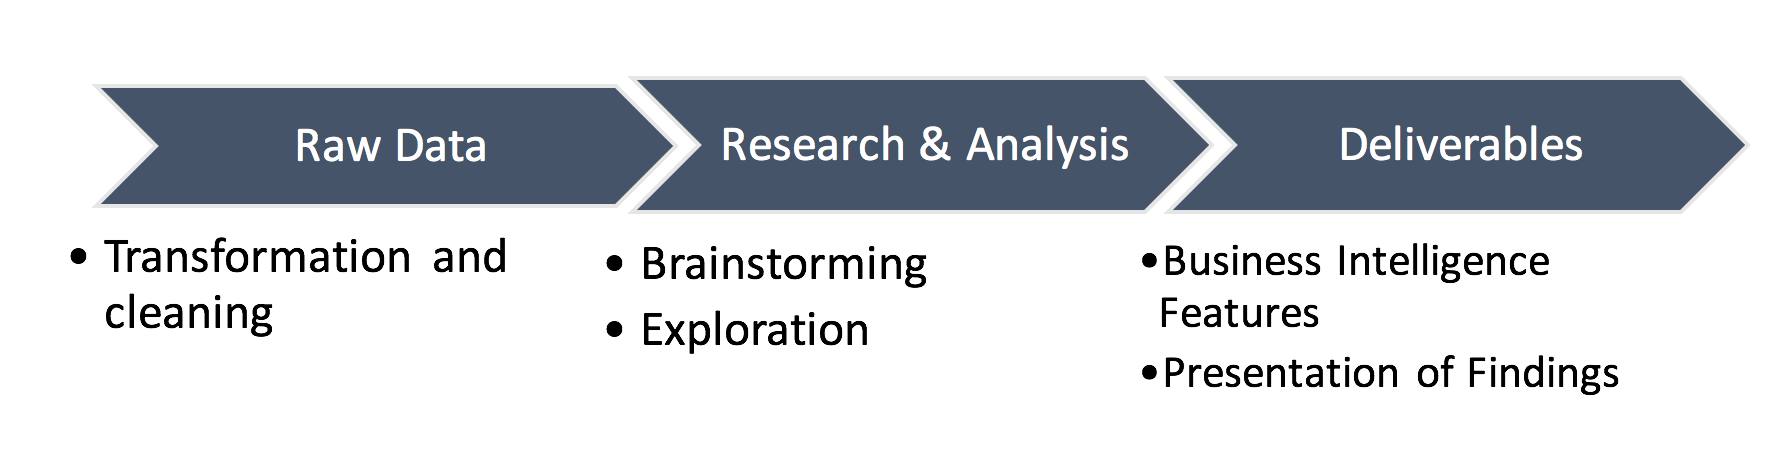
\includegraphics[width=8cm]{design_process.png}
\caption{Design process}
\end{figure}\\
\indent We start with raw data obtained from Cricsheet\cite{cricsheet} and transform it to a $csv$ format. Since data loss is inevitable, we choose to abstract attributes explicitly based upon the target audience. Our visualization caters to $2$ types of audiences
\begin{itemize}
\item A sports journalist who wants to analyze a team’s performance
\item A fan who wishes to discover trends of his/her favorite team.
\end{itemize}
Keeping it in mind, we discover the relevant insights they would be interested in. Some of them could be
\begin{itemize}
\item Analyze a player’s contribution to the team’s success.
\item Identify players in a certain bracket.
\item Team vs Team metrics
\item Compare the performance of players against different oppositions.
\end{itemize} 
\indent A good visualization is one which has interactivity and makes the comparison engaging. We present the viewer with data controls and let them uncover things on their own. Based upon these reasonings we follow $2$ main design principles. Firstly, the user should be able to select the teams to compare. Secondly, the user should be able to interact with the visualization to get additional insights in his area of interest.\\

\indent As per the guidelines of Kuchinsky et al. \cite{multipleviews} multiple views are used when there is diversity in attributes and level of abstraction. It was also recommended to use Multiple views when different view brings out correlation or disparity or when we want to break down the complex data into multiple manageable chunks and provide insights. In our cricket data, we have attributes like player names, player country, runs scored etc. where the attributes are very diverse and we have different level of abstraction at game level and at player level. Although the dimension of data is not very high, we want to break it down to provide insights of game. And hence we have chosen to use multiple views instead of using single view and overwhelm the user.\\

\indent Kuchinsky et al. \cite{multipleviews} has suggested the way in which multiple views can be used. Our system is in consistent with the rules specified and we have placed multiples views close to each other to optimize time and space and views are kept consistence.\\

\indent The multiple views which we have provided are not isolated, but they have relationship between them. These relationships are utilized by co-ordination. ``Coordination is apparent foremost when user interaction comes into play''.\cite{multipleviews2} Maximilian Scherr in his paper ``Multiple and coordinated views in Information Visualization''\cite{multipleviews2} talks about the work of North and Schneiderman’s Snap-together visualization\cite{snap} where they talk about the way to give a user the ability to explore the data and coordination between the views.\\ 

\indent According to this model, the system need to have a relational database and user is given opportunity to query the database and once he does that, the existing views should be updated. Coordination is done by bringing all the updated visualization together and creating a snap version of the system. Although our system doesn't have relational database at back end, we have created multiple files on which the user can query. Based on the user's query, we load the appropriate file and update the views of each visualization and present the snap of the system to user.\\

\indent The outcome of the matches will be win or lose, which are categorical variable but can be thought of binary variables. For the variables which are binary in nature, we used binary color scheme which differs in the hue.\cite{colorscheme}


\section {System}

\subsection {Data}
\indent A single game of Cricket generates a huge amount of data. One game of two teams consists of three hundred deliveries divided into fifty overs each. Each delivery can result into scoring runs ranging from zero to six scored by eleven different batsmen. We can aggregate this data at many levels along this hierarchy and create several interactive visualizations. The user is served into exploring data with respect to a particular team against an opponent. For example, we can explore the insights when Australia plays against India. We leverage the ball by ball data obtained from Cricsheet\cite{cricsheet}. From this data we extract the outcome of each game, teams involved, and the runs scored by each player over the years. This creates a large collection of data for several players and teams. For example, we get a data on over $30,000$ different innings played over the time. Furthermore, this data is annotated by attributes like balls faced and runs scored.\\

\indent Limited by the scope of this project, we focus only on the runs scored by a team and a batsmen as it has been proved to affect the outcome of a game. `\textit{Strike Rate}' is a major factor which determines the performance of the player and is defined as:
\begin{equation*}
Strike\ Rate = \frac{Runs\ Scored}{Balls\ Faced}
\end{equation*}

\subsection {Implementation}
We  performed  several  tests  to  analyze  the performance  and  behavior  of  several  of  our  design decisions   and   our   prototype   implementation.   Our
prototype  system  was  written  as  a  JAVASCRIPT application using D3\cite{d3} and C3\cite{c3} libraries and some helper libraries like `d3-queue'\cite{q} to resolve asynchronous issues.  Our prototype was tested in a  machine  with  an  Intel  i5-3770k  processor,  8GB  of RAM,  Google Chrome browser and  an  NVIDIA  GTX  670  graphics  card,  all under Windows 7 64-bit

\subsection {Layout}
Our system is comprised of four modules that visualize team and player performance. We have primarily used the number of runs scored as the metric to measure the performances of the players as well as the impact it has on the overall performance of the team. In our system, we provide the user with two drop-down menus, that list the names of the various cricket playing nations. These drop downs provide an effective way of filtering the results based on a team and the opposition it has played against. The first drop-down allows users to select a country for which they would like to view the team and player performances, the second, optional drop-down allows users to narrow results by selecting a single country that has played against the first country. By default the second drop down is set to show the results against all the oppositions.


\subsection {Views}

\subsubsection {Bar charts}
The first visualization contains two parallel bar charts (positioned one below another) which can be used to analyze a team’s performance using their runs score. The first chart shows the number of runs scored by the team in a time-line fashion. The x-axis contains an ordinal scale with match dates while the y-axis contains the scores (runs). The second chart shows the margin by which the team has won or lost in each match. The length of the each bar in both charts represents the score or margin respectively. In case the team won the match while batting second, the margin is taken to be one. The color of each bar shows whether the match was won or lost. \\

\indent The visualization also has a sorting feature which allows users to sort matches by date, runs score, or margin of runs scored. The sorting mechanism is useful and really effective in arriving at the conclusions such as, what is a safe score for a team if batting second, what is the probability that a team would successfully defend or chase a target set by the opposition. \\

\indent Filtering based on the margin of runs helps us understand whether the team plays too many close games. This could be due to the fact that the team loses out in the critical points in the game. South Africa for instance has always had the tag of being ``Chokers'' as they have been known to be a team that loses important matches at in-spite of being one of the best teams in the world.\\

\indent Another valuable insight that can be derived by sorting the data based on the margin is to gaze whether the team's performance has been increasing, if the margins have been decreasing, or vice versa.\\

\indent Using these sorting features along with the second drop down to select the opposition, can help us understand how the team has been performing against different oppositions. Fig \ref{fig:bar_chart} shows a bar chart for India\\ \\ 

\begin{figure}[ht]
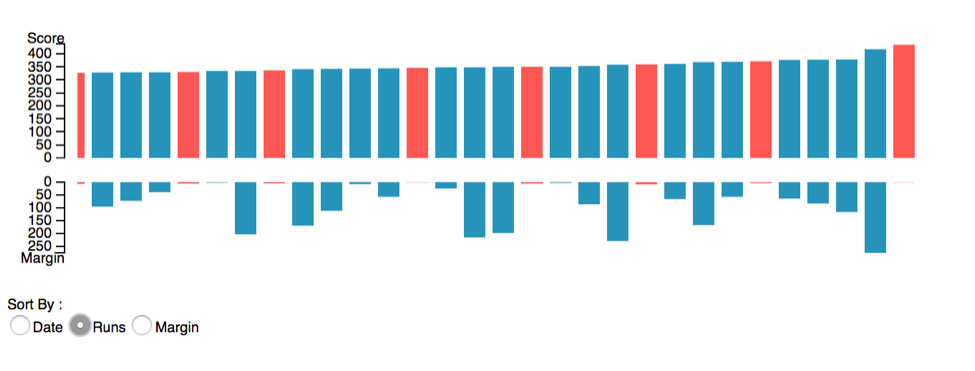
\includegraphics[width=9cm]{bar_chart.png}
\caption{Bar chart for Team India}
\label{fig:bar_chart}
\end{figure}

The next two visualizations in our system combine to make a multiple linked view. Using the data visualization technique of brushing, we linked a scatter-plot with a histogram.
 
\subsubsection {Scatter-plot}
A scatter-plot is used to depict the relationship between the number of balls faced by a batsman in innings and the runs they scored. The x-axis contains the number of balls in an inning faced by the batsmen and the y-axis contains the number of runs scored. The relationship between these two values is known as a ``strike rate'' in cricket. Scoring a lot of runs in the game is as important as the number of balls faced in scoring those runs. Thus, the players who score a lot at an extremely fast rate are considered to be more valuable players when compared to players who make a lot of runs at a slower rate. Essentially, each point in the scatter-plot will represent an inning played by player in terms of their strike rate. \\ Fig \ref{fig:scatter_plot} shows the scatter-plot for each innings played by the players of Team India.

\begin{figure}[ht]
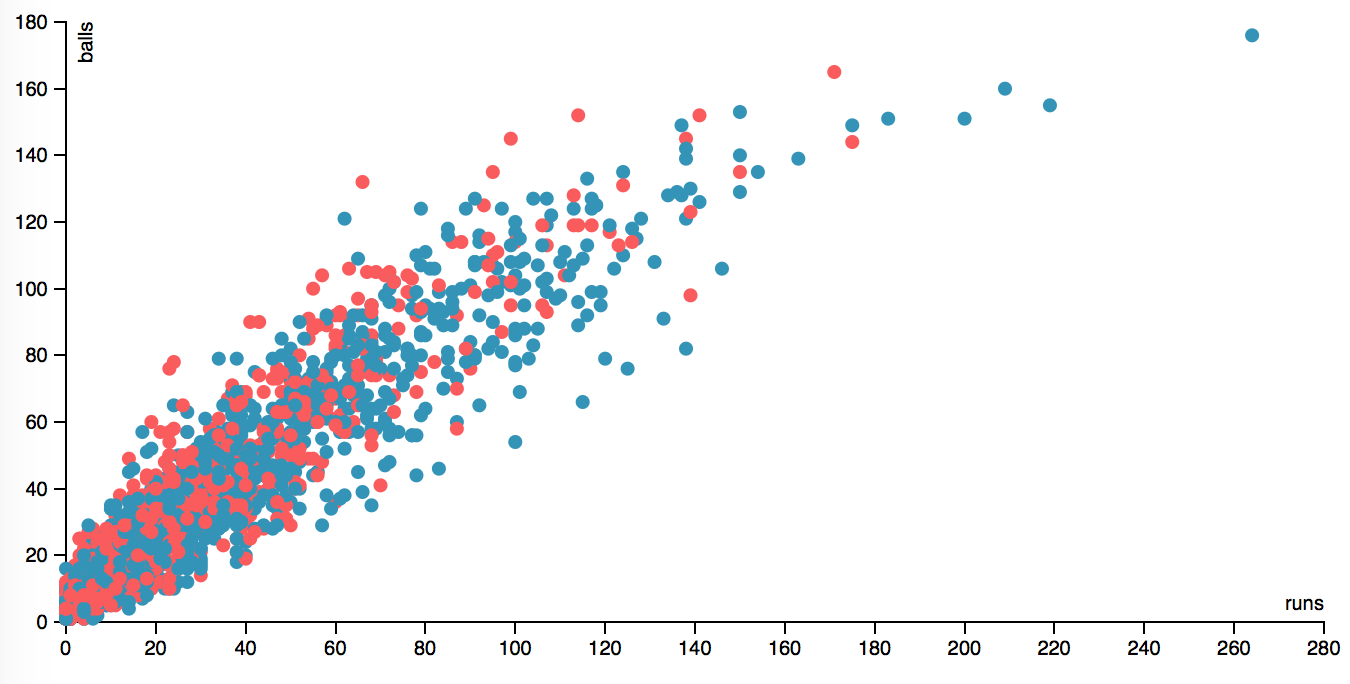
\includegraphics[width=9cm]{scatter_plot.png}
\caption{Scatter-plot for Team India}
\label{fig:scatter_plot}
\end{figure}

\indent The points in the scatter-plot are color-coded; the color of a point represents the outcome of the match in which the inning (i.e. the point of interest) was played. Blue is used to represent a win while red is used to represent a loss. For example, a point depicting the strike rate of Player A will be blue if the team had won the particular match. Color-coding the scatter-plot help us find an underlying relationship between a player’s performance and the outcome of the match.\\

\indent On each point in the scatter-plot, we show a tool-tip which gives additional information such as the corresponding player name, the player’s runs scored, and the number of balls faced by the player.\\

\indent The scatter-plot also has an option to select a range of points (brushing). When a set of points is selected in the scatter-plot, a dataset is generated with all the points in the selected area and passed to a histogram. that would visualize a stacked bar graph for each player for whom a point is found in the selection. The stacked bar will represent the number of points in the selected area for a lost cause vs winning cause for a player. Fig \ref{fig:scatter_plot_brushing} shows the brushing feature in the scatter-plot.

\begin{figure}[ht]
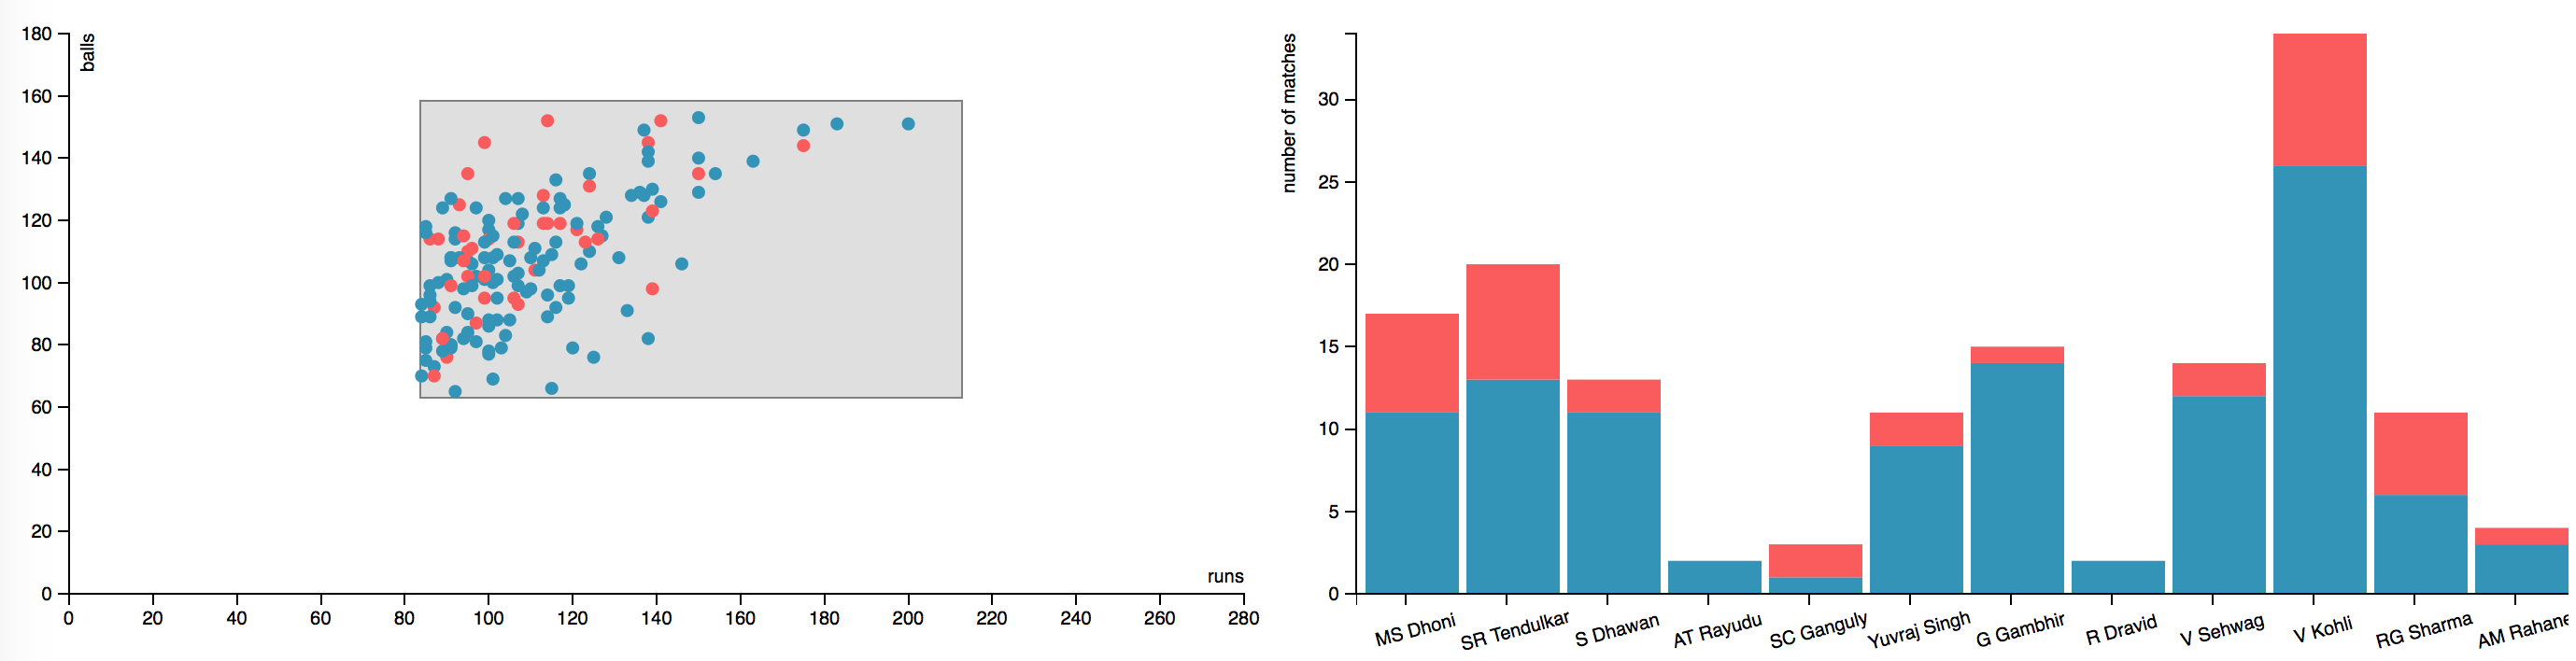
\includegraphics[width=9cm]{scatter_plot_brushing.png}
\caption{Brushing in scatter plot}
\label{fig:scatter_plot_brushing}
\end{figure}


\subsubsection {Stacked Bar}
The stacked bar chart is designed to visualize player frequencies that will be retrieved from the dataset mentioned above. For example, if two points are selected in the scatter-plot and both correspond with strike rates of player ``X'', the histogram will contain a bar for player ``X'' with a height of two. This visualization is aimed at understanding how a particular player's performance affects the success of his team. A stacked bar in the chart represents the count of innings found in the selection made in the data visualized in the scatter plot. Each bar will be stacked based on the number of innings that were played in a lost cause against the number of innings played where the team won the game.\\

\indent `Finishers' is a term often used to  describe  a player who has the ability to stay `not out' till the end of the game and thus himself lead the team to a win. These players often have to face the pressure situation in a game. Players like the Indian Cricket team captain \textit{Mr M.S. Dhoni} and \textit{Suresh Raina} have made a name for themselves to be one of the best finishers in the game. The visualization not only helps us verify these facts but also help us find other such players who may not have received the due credit. Fig \ref{fig:stacked_bar_chart} shows the stacked bar chart for Team India.\\

\begin{figure}[ht]
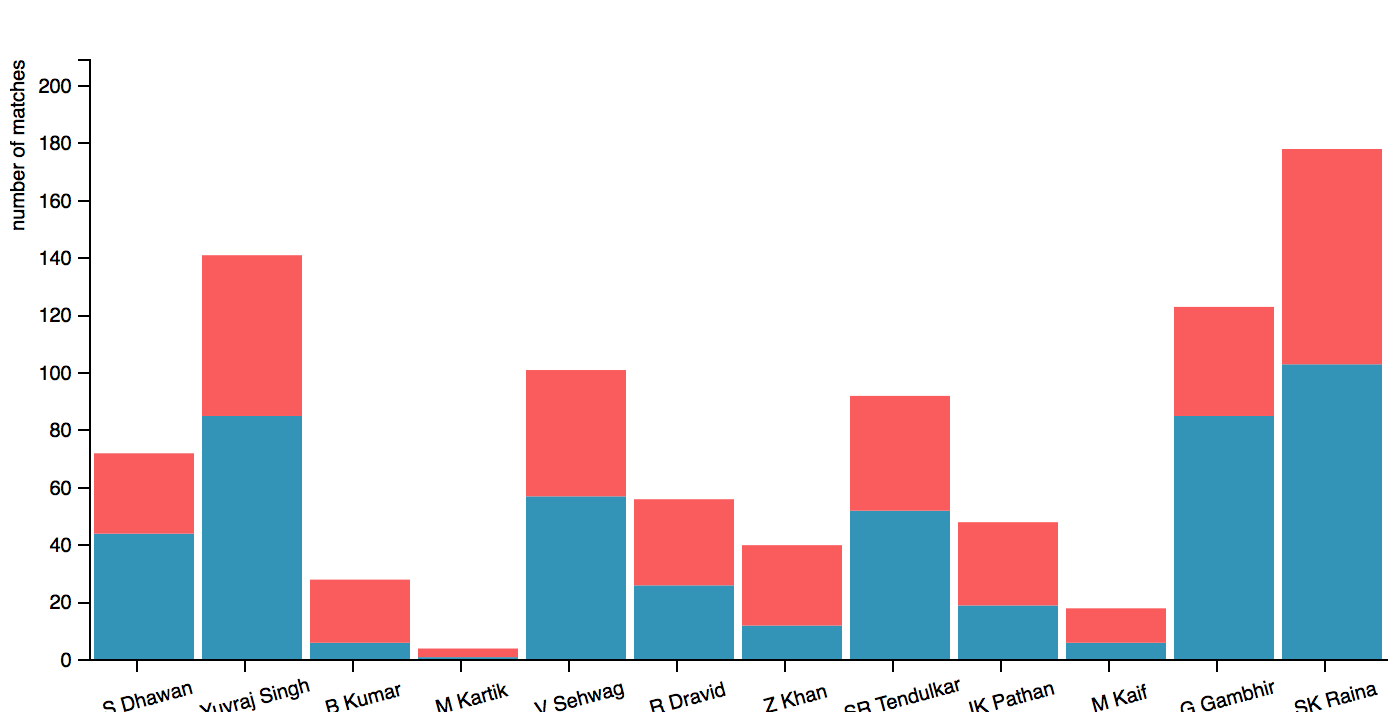
\includegraphics[width=9cm]{stacked_bar_chart.png}
\caption{Stacked Bar Chart}
\label{fig:stacked_bar_chart}
\end{figure}

\indent When used with the opposition filter, this visualization also helps us identify how certain players play against different oppositions. For instance, even though the legend \textit{Sachin Tendulkar} has higher number of runs against `Pakistan', it is actually \textit{Yuvraj Singh} whose innings have helped India win $100\%$ of games whenever he has scored a score of 80 or more in a game. Interestingly, \textit{Yuvraj Singh} has had just one inning of $80$ or more against another opposition `New Zealand'.

\subsubsection {Stacked Area Chart}
Stacked area chart is an extremely effective visualization in visualizing the performance of the team based on the sum of the number of runs, the players of the team, have been scoring each year. Stacked area chart also provides an effective means of analyzing the contribution made by a key batsman in the total number of runs scored. This visualization is useful in understanding when the team has peaked and coinciding this with the important tournaments played over the years gives us an understanding of the results of a lot them. Fig \ref{fig:stacked_area_chart} shows a stacked area chart for performance of Team India over the years.\\

\begin{figure}[ht]
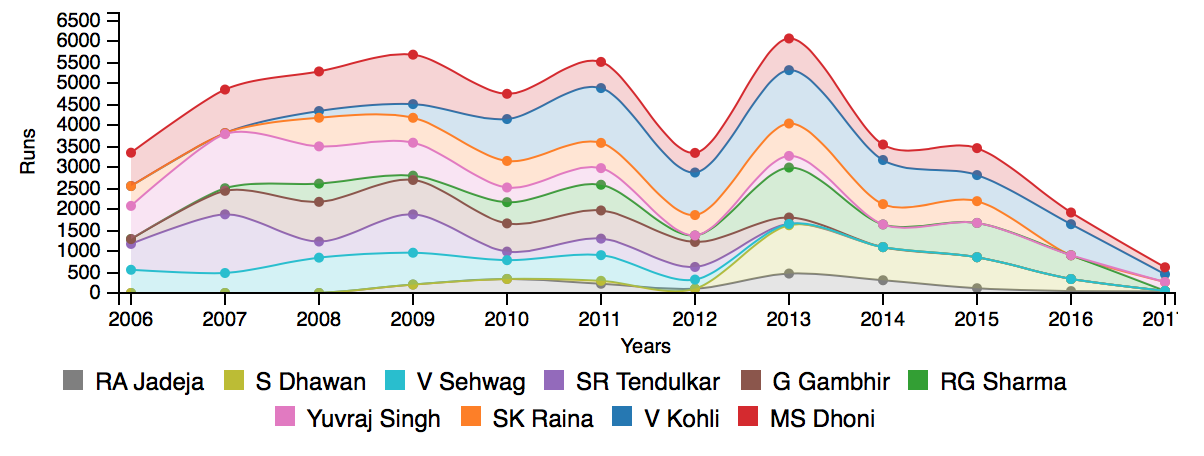
\includegraphics[width=9cm]{stacked_area_chart.png}
\caption{Stacked Area Chart for Team India}
\label{fig:stacked_area_chart}
\end{figure}

\indent For instance, team India performed really well in the years $2011$ and $2013$, the same time that they won the Cricket World cup and the ICC Champion’s trophy, two of the most prestigious trophies in cricket. If we hover over the years, we also get the details about the number of runs scored by individual players in a particular year. Fig \ref{fig:stacked_area_details} shows the run details by each player of Team India in the year 2013. New Zealand, who had an extraordinary year as a team in the year $2015$, reached the finals of the Cricket World Cup for the first time ever in the history of the tournament.\\

\begin{figure}[ht]
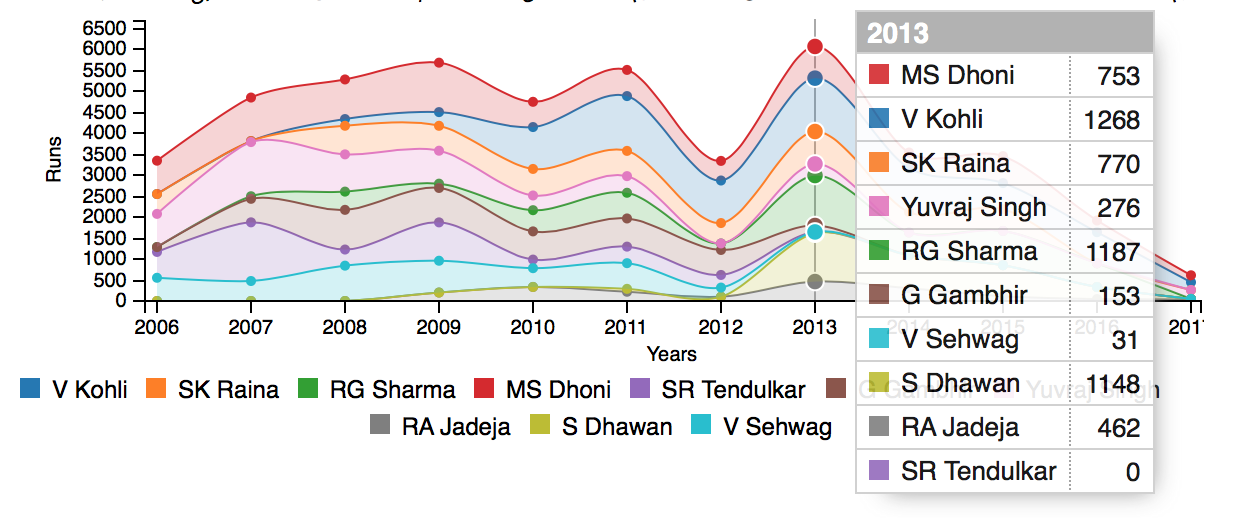
\includegraphics[width=9cm]{stacked_area_details.png}
\caption{Details on demand for Team India in 2013}
\label{fig:stacked_area_details}
\end{figure}

\indent Not only this, the visualization also helps us understand the effect that the retirement of the important players has on a team. In the year $2016$, when three of the most prolific batsmen of `Sri Lanka', \textit{Mr. M. Jayawardene}, \textit{Mr K. Sangakara} and \textit{Mr T. Dilshan} retired, their performance as a team went to an all time low in the last $10$ years.\\

\indent This visualization also helps analyze how the careers of individual players have evolved over the years. From the debuts and retirements of the players to injuries, that led to a temporary lapse in the performance of a player, can all be visualized using this visualization.

\section {Results}
The complete system has an overview of all the views consolidated into one and is presented as shown in Fig \ref{fig:overview}.

\begin{figure}[ht]
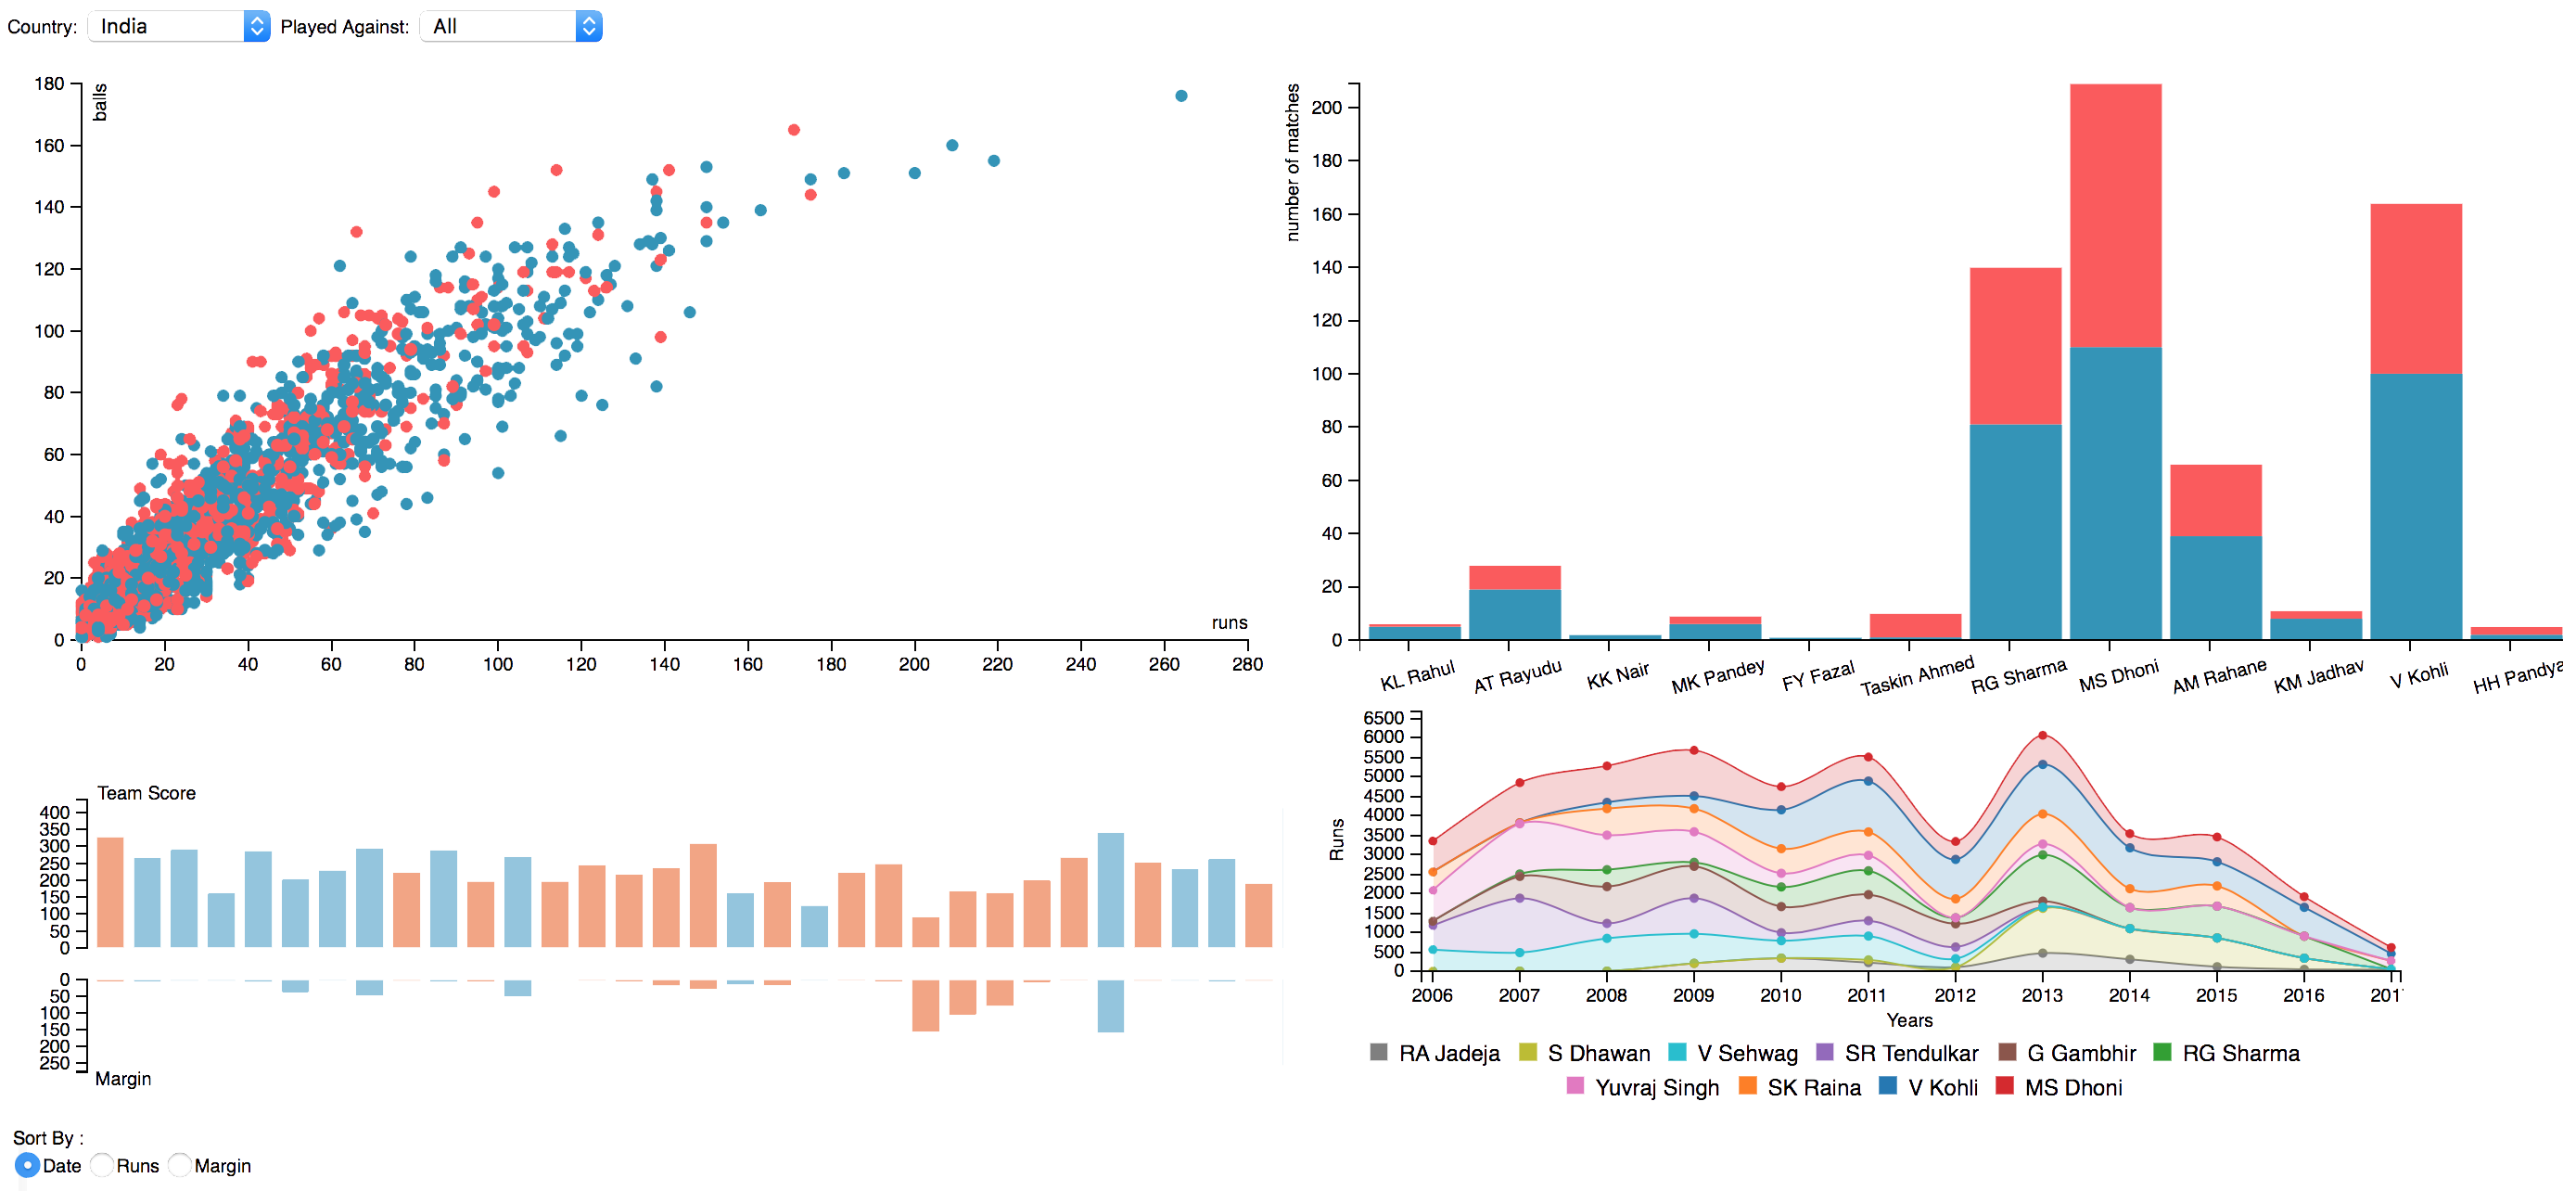
\includegraphics[width=9cm]{overview.png}
\caption{System overview : In the top left corner we have an option to select the home country and the opponent. The scatter plot shows each innings played by the player over the period of 2006-2017. Red dots represent a loss, while blue represents a win. The histogram tells us which players have been playing dominantly for a country. The bar chart gives an insight for each game played, while the stacked area chart visualizes the performance of the team throughout the years.}
\label{fig:overview}
\end{figure}

% An example of a floating figure using the graphicx package.
% Note that \label must occur AFTER (or within) \caption.
% For figures, \caption should occur after the \includegraphics.
% Note that IEEEtran v1.7 and later has special internal code that
% is designed to preserve the operation of \label within \caption
% even when the captionsoff option is in effect. However, because
% of issues like this, it may be the safest practice to put all your
% \label just after \caption rather than within \caption{}.
%
% Reminder: the "draftcls" or "draftclsnofoot", not "draft", class
% option should be used if it is desired that the figures are to be
% displayed while in draft mode.
%
%\begin{figure}[!t]
%\centering
%\includegraphics[width=2.5in]{myfigure}
% where an .eps filename suffix will be assumed under latex, 
% and a .pdf suffix will be assumed for pdflatex; or what has been declared
% via \DeclareGraphicsExtensions.
%\caption{Simulation results for the network.}
%\label{fig_sim}
%\end{figure}

% Note that IEEE typically puts floats only at the top, even when this
% results in a large percentage of a column being occupied by floats.
% However, the Computer Society has been known to put floats at the bottom.


% An example of a double column floating figure using two subfigures.
% (The subfig.sty package must be loaded for this to work.)
% The subfigure \label commands are set within each subfloat command,
% and the \label for the overall figure must come after \caption.
% \hfil is used as a separator to get equal spacing.
% Watch out that the combined width of all the subfigures on a 
% line do not exceed the text width or a line break will occur.
%
%\begin{figure*}[!t]
%\centering
%\subfloat[Case I]{\includegraphics[width=2.5in]{box}%
%\label{fig_first_case}}
%\hfil
%\subfloat[Case II]{\includegraphics[width=2.5in]{box}%
%\label{fig_second_case}}
%\caption{Simulation results for the network.}
%\label{fig_sim}
%\end{figure*}
%
% Note that often IEEE papers with subfigures do not employ subfigure
% captions (using the optional argument to \subfloat[]), but instead will
% reference/describe all of them (a), (b), etc., within the main caption.
% Be aware that for subfig.sty to generate the (a), (b), etc., subfigure
% labels, the optional argument to \subfloat must be present. If a
% subcaption is not desired, just leave its contents blank,
% e.g., \subfloat[].


% An example of a floating table. Note that, for IEEE style tables, the
% \caption command should come BEFORE the table and, given that table
% captions serve much like titles, are usually capitalized except for words
% such as a, an, and, as, at, but, by, for, in, nor, of, on, or, the, to
% and up, which are usually not capitalized unless they are the first or
% last word of the caption. Table text will default to \footnotesize as
% IEEE normally uses this smaller font for tables.
% The \label must come after \caption as always.
%
%\begin{table}[!t]
%% increase table row spacing, adjust to taste
%\renewcommand{\arraystretch}{1.3}
% if using array.sty, it might be a good idea to tweak the value of
% \extrarowheight as needed to properly center the text within the cells
%\caption{An Example of a Table}
%\label{table_example}
%\centering
%% Some packages, such as MDW tools, offer better commands for making tables
%% than the plain LaTeX2e tabular which is used here.
%\begin{tabular}{|c||c|}
%\hline
%One & Two\\
%\hline
%Three & Four\\
%\hline
%\end{tabular}
%\end{table}


% Note that the IEEE does not put floats in the very first column
% - or typically anywhere on the first page for that matter. Also,
% in-text middle ("here") positioning is typically not used, but it
% is allowed and encouraged for Computer Society conferences (but
% not Computer Society journals). Most IEEE journals/conferences use
% top floats exclusively. 
% Note that, LaTeX2e, unlike IEEE journals/conferences, places
% footnotes above bottom floats. This can be corrected via the
% \fnbelowfloat command of the stfloats package.




\section{Conclusion}
We tried to present a system following the visual information-
seeking  mantra\cite{mantra}  of  `Ben  Shneiderman'  to  analyze  a  team's match plan. Therefore, we proposed appropriate analysis and
visualization techniques for the different steps of ``overview
first'' (Scatter Plot), ``zoom and filter'' (Brushing and sorting bar chart), then ``detail-on-demand'' (Histogram and stacked area chart). We focused on the fixed parameter of strike rate of a player. However, there still exists a challenge to extract information and gain insights from bowling statistics of a team. Some teams are known for exceptional spinners and we have players who are capable of conceiving all the wickets in a game. Such players also impact the outcome of a game, and as a future work we plan to integrate bowling information also in this visualization.\\

\indent Interaction between the visualizations is a crucial part of our prototype. We integrated methods to analyze player performances over the time but we may also  need  to  search  for  similar  player  behavior  on  more abstract levels. We may want to know how players adapt their behavior when playing with other players. A partnership between two players can be a very interesting area of analysis. \\

\indent Apart from the players, the team behavior and strategy as a whole could also be one important metric to consider. A team could play offensive under one captain while defensive under the other one. We may want to know how players perform under these kind of conditions. At this point it is unclear how can be we visualize a strategy or a tactic. Doing a sentiment analysis could be a potential first step towards this open problem.

\bibliographystyle{plain}
\bibliography{bibliography.bib}


\end{document}